\chapter{Conversion from \protect\LaTeX\ to HTML}
\label{ch:latex-to-html}

\section{Choosing your preferred workflow}

There are several tools available to perform conversion of \LaTeX\ to HTML. Here, we focus on \href{https://vlmantova.github.io/bookml/}{BookML}, which uses \href{https://math.nist.gov/~BMiller/LaTeXML/}{LaTeXML} in the background; note that this is the same technology used by \href{https://info.arxiv.org/about/accessible_HTML.html}{arXiv} to produce HTML versions of research papers from the \verb|.tex| source.

There are three steps to converting LaTeX notes to HTML using BookML:
\begin{enumerate}
    \item write notes in \LaTeX{};
    \item use BookML to convert \LaTeX{} code to HTML;
    \item share the HTML version with students.
\end{enumerate}
Your precise workflow will depend on how you wish to share the HTML version with students and whether you prefer to work in Overleaf, with GitHub or on your local machine. Some possible workflows are summarised in the figure below.


\begin{figure}[h]
    \centering
    \iflatexml
        
\includegraphics{img/process.svg}
    \else
        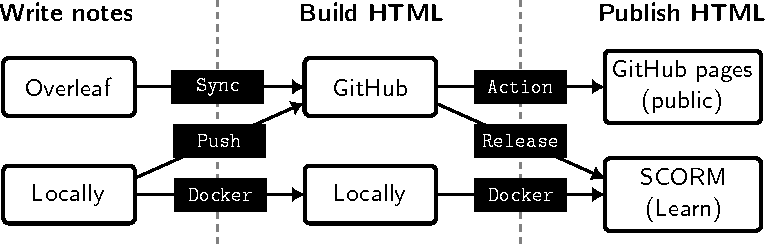
\includegraphics{img/process.pdf}
    \fi
    \caption{Workflow options to build HTML course materials.}
    \alttext{Flowchart showing different workflow options to build HTML course materials. TODO: improve alt text}
    \label{fig:workflow}
\end{figure}

We give details of two of these workflows below. You may wish to deviate from these documented workflows if you feel comfortable doing so. 


\section{Overleaf \textrightarrow{} GitHub \textrightarrow{} GitHub Pages}

If you are happy to write your \LaTeX{} notes in Overleaf, to have your source code stored (privately) on GitHub and to have your HTML notes available on a public website then the \textbf{Overleaf \textrightarrow{} GitHub \textrightarrow{} GitHub Pages} workflow will likely be most convenient. After the initial setup, there is no need to interact directly with GitHub.

\begin{enumerate}[align=left]
    \item[Step 1:] Make a copy of the course notes template from GitHub
    \item[Step 2:] Create an Overleaf project linked your GitHub repository
    \item[Step 3:] Write your notes in Overleaf and sync with GitHub
\end{enumerate}


\subsection{Step 1: Make a copy of the course notes template from GitHub}

\subsubsection{Create a GitHub account and join the UoE School of Mathematics organization}

If you already have a GitHub account then please  \href{mailto:lt@maths.ed.ac.uk?subject=Please%20add%20me%20to%20SoM%20GitHub%20organization}{email the Learning Technology Team lt@maths.ed.ac.uk} giving your GitHub username and ask to be added to the UoE School of Mathematics GitHub organization. 

If you do not have a GitHub account then please \href{mailto:lt@maths.ed.ac.uk?subject=Please%20add%20me%20to%20SoM%20GitHub%20organization}{email the Learning Technology Team lt@maths.ed.ac.uk} and ask for an invitation to the UoE School of Mathematics GitHub organization. You will receive an email from GitHub with a link to create an account and join the SoM organization. Please note that the email may not render properly in your mail client -- the link may appear as an empty box but this is the invitation link!

\begin{figure}[h]
    \centering
    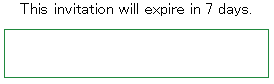
\includegraphics{img/GitHub-invitation.png}
    \caption{GitHub invitation link when it appears empty.}
    \alttext{A blank rectangular box with the text ``This invitation will expire in 7 days'' written above.}
    \label{fig:gh-invitation}
\end{figure}


\subsubsection{Make a new GitHub repository for your notes using the SoM template}

Sign in to your GitHub account and \href{https://github.com/UoE-School-of-Mathematics/BookML-Workflow-Template}{visit the template repository}.
Click the ``Use this template'' button at the top right of the page.

\begin{figure}[h]
    \centering
    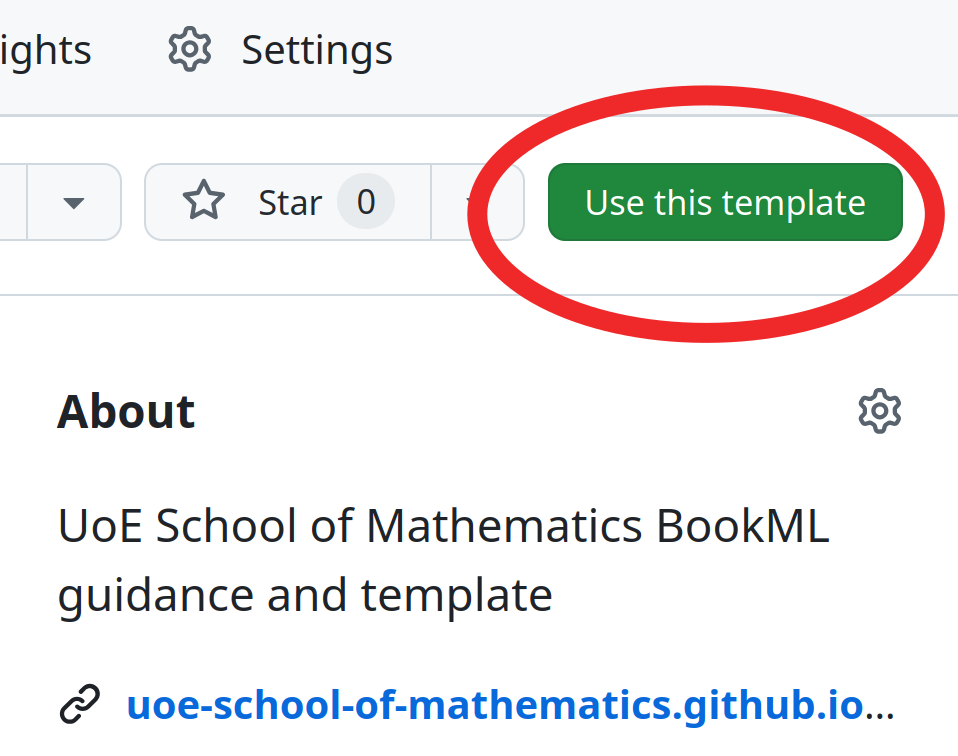
\includegraphics[width=0.5\textwidth]{img/use_template.png}
    \caption{``Use this template'' button is at the top right of the page.}
    \alttext{A screenshot of a webpage showing a green ``Use this template'' button circled in red.}
    \label{fig:use-template}
\end{figure}

The ``Create a new repository'' page has some options -- the defaults are fine. \textbf{Please ensure you the box to ``Include all branches'' is NOT ticked.} By default, your notes will be stored in a private repository on GitHub in the UoE School of Mathematics organization. You are free to change these settings if you wish.

Choose an appropriate repository name; we recommend that you choose your \textbf{course abbreviation} (e.g. FAC, IMU, IDS, FPM\ldots), or include it in the name.

Please wait at least 3~minutes before moving on. GitHub needs some time to initialise the project.

\subsubsection{Set up the automatic creation of a website for your HTML notes}

You can set up a GitHub Action to automatically generate the HTML version of your notes from the GitHub repository, and keep this up to date. This means you only need to add a link to your notes on Learn once and this will always point to the most up-to-date version of your notes.

To set up a publicly-accessible website with your HTML notes in GitHub, first visit your new repository in GitHub. In the top menu click \textbf{Settings} then \textbf{Pages} in the left menu.

Under \textbf{Build and deployment}, look for the \textbf{Branch} option. From the \textbf{Select branch} option, choose \texttt{gh-pages} and \textbf{Select folder} \texttt{/docs}.

\begin{figure}[h]
    \centering
    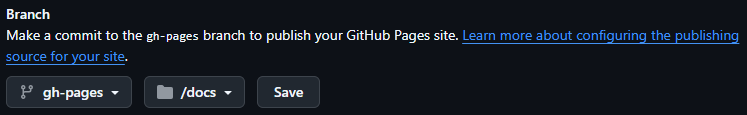
\includegraphics[width=\columnwidth]{img/GitHub-Pages.png}
    \caption{Select the \texttt{gh-pages} branch and the \texttt{/docs} folder.}
    \alttext{A screenshot of a section of the ``Settings'' page. The text reads ``Branch: Make a commit to the gh-pages branch to publish your GitHub Pages site.'' Two drop-down menus and a ``Save'' button are below. The first drop-down menu shows the option ``gh-pages'' was picked. The second shows the option ``/docs''.}
    \label{fig:gh-pages}
\end{figure}

Wait 1~minute then refresh the page. You should now see a link to the publicly-available site hosting your HTML notes. This includes the URL that you should use to share your notes with students.

\begin{figure}[h]
    \centering
    
\includegraphics[width=\columnwidth]{img/GitHub-site-link.png}
    \caption{The link to your course site.}
    \alttext{A screenshot of a section of the ``Settings'' page. The text reads: ``Your site is live at https://uoe-school-of-mathematics.github.io/ohagan_demo/'', then ``Last deployed by sohagan1 last month''. There is a ``Visit site'' button on the right.}
    \label{fig:gh-site-link}
\end{figure}


\subsection{Step 2: Create an Overleaf project linked your GitHub repository}

\subsubsection{Link your Overleaf account to your GitHub account}

Visit your \href{https://www.overleaf.com/user/settings}{Overleaf account settings}. Under \textbf{Project Synchronisation}, click \textbf{Link} next to \textbf{GitHub Sync}. Follow the prompts to link Overleaf and GitHub.

\subsubsection{Make an Overleaf project from your GitHub repository}

At this stage you should have a GitHub repository created from the SoM template.

In Overleaf, create a new project ensuring you choose \textbf{Import from GitHub}. Then choose \textbf{Import to Overleaf} for the appropriate repository.

\begin{figure}[h]
    \centering
    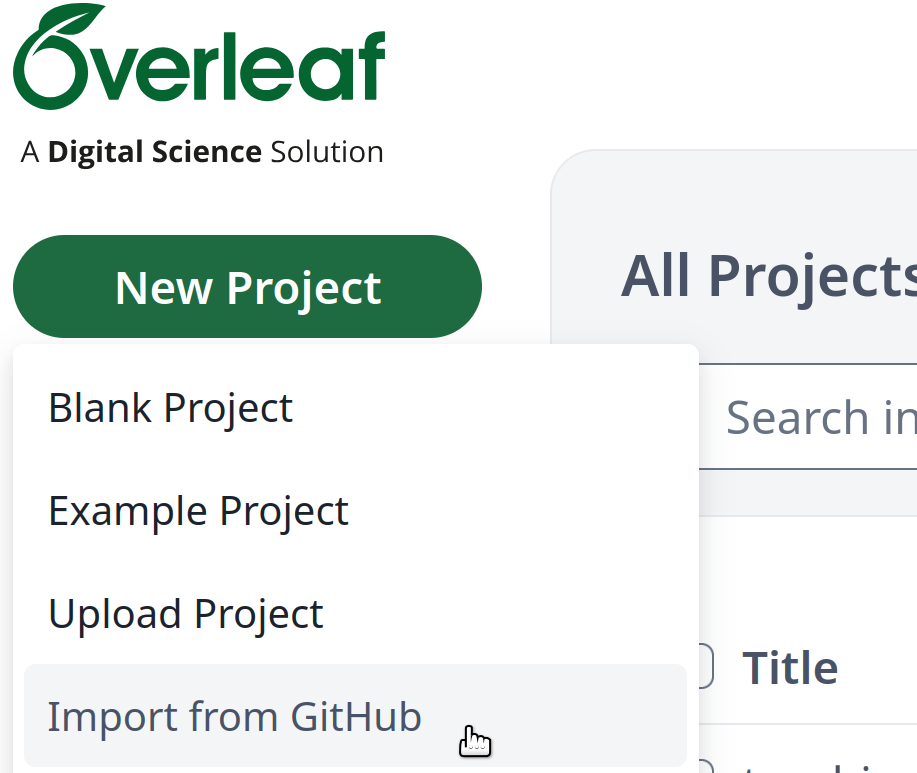
\includegraphics[width=0.5\textwidth]{img/overleaf_new.png}
    \caption{Choose ``Import from GitHub'' when creating the new project.}
    \alttext{A screenshot of the Overleaf ``New project'' options, showing ``Import from GitHub'' selected by the user.}
    \label{fig:gh-overleaf-new}
\end{figure}

Once this is complete, you should see a copy of this documentation in your own Overleaf project.


\subsection{Step 3: Write your notes in Overleaf and sync with GitHub}

At this stage you should have an Overleaf project for your notes, linked to your GitHub repository, and have an action set up to automatically build a public website with the HTML version of your notes.

Now you can work on your notes just like any other Overleaf project.

Whenever you want to publish changes to the HTML version, you need to push the changes to your GitHub repository. To do this, in Overleaf, click \textbf{Menu} (top left) and then choose \textbf{GitHub} under the \textbf{Sync} menu.

\begin{figure}[h]
    \centering
    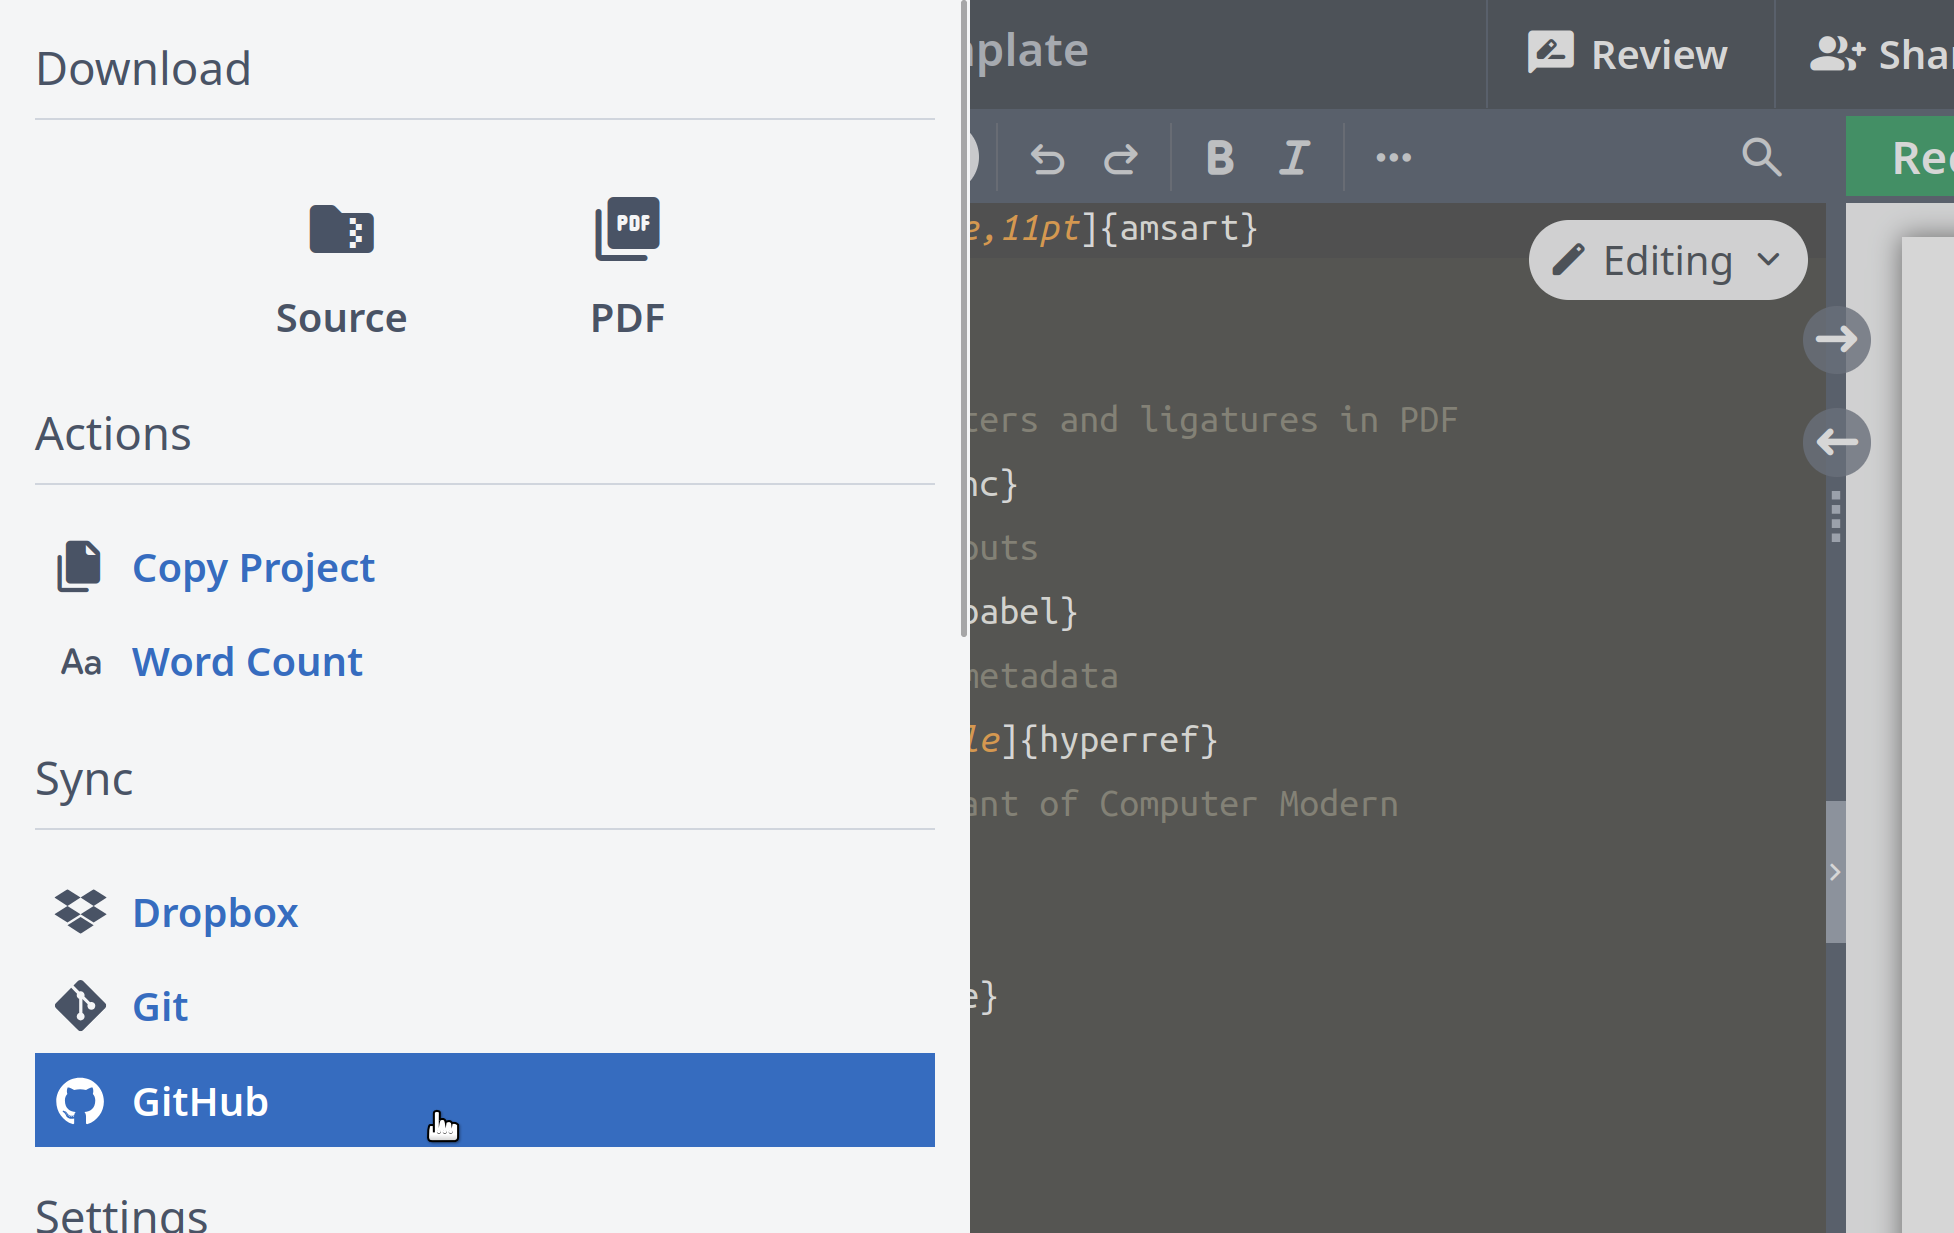
\includegraphics[width=0.6\textwidth]{img/overleaf_sync.png}
    \caption{The ``GitHub'' option in the Overleaf top-left menu.}
    \alttext{A screenshot of the Overleaf menu bar, showing ``GitHub'' selected by the user.}
    \label{fig:gh-overleaf-sync}
\end{figure}

Click \textbf{Push Overleaf changes to GitHub}, enter a description of the changes you have made (optional) and then click \textbf{Sync}.

Behind the scenes, GitHub will now rebuild the HTML version of your notes and update the public website. You don't need to interact directly with GitHub again.


\section{Locally \textrightarrow{} Locally \textrightarrow{} SCORM}

\subsection{Using Docker}
\label{ssec:docker}

To run BookML, we can use a Docker container --- a lightweight, portable unit that packages an application and all its dependencies, ensuring that it runs consistently across different environments. This removes the need to download software and maintain dependencies on your computer.

Importantly for us: there is a \href{https://github.com/vlmantova/bookml/pkgs/container/bookml}{Docker image available for BookML}, which is ready-to-use and contains everything we need.

To use it, we can use Docker Desktop, which is available for Windows and Mac, or Docker Engine, which is available for Linux. An open-source alternative (compatible with Docker) is Podman, which is available for Windows, Mac, and Linux. In any case, the key steps are:

\begin{enumerate}
    \item Setup (just once): install Docker or Podman, and download the Docker image.
    \item Convert: run a single command in the folder with your \verb|.tex| files.
\end{enumerate}

Both Docker and Podman allow us to use either the command line or a graphical interface. If you don't know which one to choose, just pick one and try it!

\noindent \textbf{Notes: }
\begin{itemize}
    \item If you have a managed Windows machine, Docker Desktop is available from the software centre. This is a slightly complicated process, 
    see Appendix \ref{app:a} for instructions. It may be simpler to request `Make Me Admin' and install from the internet.\textcolor{red}{TODO}
    If you wish to use Podman, you will need to request `Make Me Admin'.
    \href{https://www.ed.ac.uk/information-services/computing/desktop-personal/supported/windows-10/makemeadmin}{Guidance on `Make Me Admin'}.
    \item The Learning Technology team will be able to assist you with installing Docker or Podman --- email \verb|lt@maths.ed.ac.uk| to ask for help.
\end{itemize}

\subsubsection{Setup (first-time only)}
\label{sssec:setup}

\paragraph{Option 1 - to set up Docker:}

\begin{enumerate}
    \item
        \begin{itemize}
            \item \textbf{Windows/MacOS/Linux:} \href{https://docs.docker.com/desktop/install/windows-install/}{Download Docker Desktop from \textbf{this} link} or the Software Centre, and install as instructed by the interface. Launch Docker Desktop. 
There are versions of the download file of Docker Desktop which cause an error. Ensure you are downloading the version that is listed in the documentation.
            \item \textbf{Alternatively for Linux only:} Download and install Docker Engine, following \href{https://docs.docker.com/engine/install/}{the instructions for your distribution}.
        \end{itemize}
    \item Launch a terminal (use \verb|cmd.exe| on Windows), and run the command:\\
        \verb|docker pull ghcr.io/vlmantova/bookml:latest|\\
        This will download the Docker image to your machine.
\end{enumerate}

\paragraph{Option 2 - to \href{https://podman.io/docs/installation}{set up Podman}:}

Note that this requires ``Make Me Admin'' on Windows managed machines.

\begin{enumerate}
    \item \href{https://podman.io/}{Download Podman Desktop from here} and install as instructed by the interface. 
    \item Podman desktop will open, and you will be asked to setup.
    Click the `Setup' button and follow through the instructions 
    that follow. When prompted, select `Yes', and then `Install'. 
    \item Once fully installed, we can download the image. To do this, open the `Images' tab
        (the 4th option on the left-hand side of the screen) and click \verb|Pull| on the top right of the screen, then enter \verb|ghcr.io/vlmantova/bookml:latest| and click ``Pull image''. 
\end{enumerate}

\subsubsection{Conversion}
\label{sssec:conversion}

Before you start, for better results, add \verb|\usepackage{bookml/bookml}| to the preamble of your \verb|.tex| file(s) (after the \textbackslash\verb| documentclass{...}| command). This is not necessary, if using the template provided by the School of Mathematics. This package may cause an error in overleaf, unless you upload the BookML folder to your project.

\paragraph{Option (a) - using the command line:}

\begin{enumerate}
    \item Start a terminal in the directory containing your \verb|.tex| file(s). (Use \verb|cmd.exe| in Windows.)
    \item Run the command:\\
        \verb|{software} run -t -v .:/source ghcr.io/vlmantova/bookml:latest|\\
        (replace \verb|{software}| with \verb|docker| or \verb|podman|).
\end{enumerate}

\paragraph{Option (b) - using the graphical interface:}

\begin{enumerate}
    \item In Docker/Podman Desktop, click on the `Images' tab, and you will see the image you have just downloaded. Click the `Play' button (Figure~\ref{fig:docker_desktop_run}).
    \item Under ``Volumes'', specify the ``Host path'' to be the path to your folder, and the ``Container path'' to be \verb|/source|. (In Docker Desktop, this is under ``Optional settings'' -- see Figure~\ref{fig:docker_desktop_path}.)
    % \item In `Optional settings', under `Volumes', in the left box called \verb|Host Path|, copy the path to your folder, or click the three dots to navigate to the folder. In the right box labelled `Container Path', type \verb|/source|.
    \item Click `Run' (Docker) or `Start Container' (Podman) to produce the PDF and HTML outputs.
\end{enumerate}

\begin{figure}[h!]
    \centering
    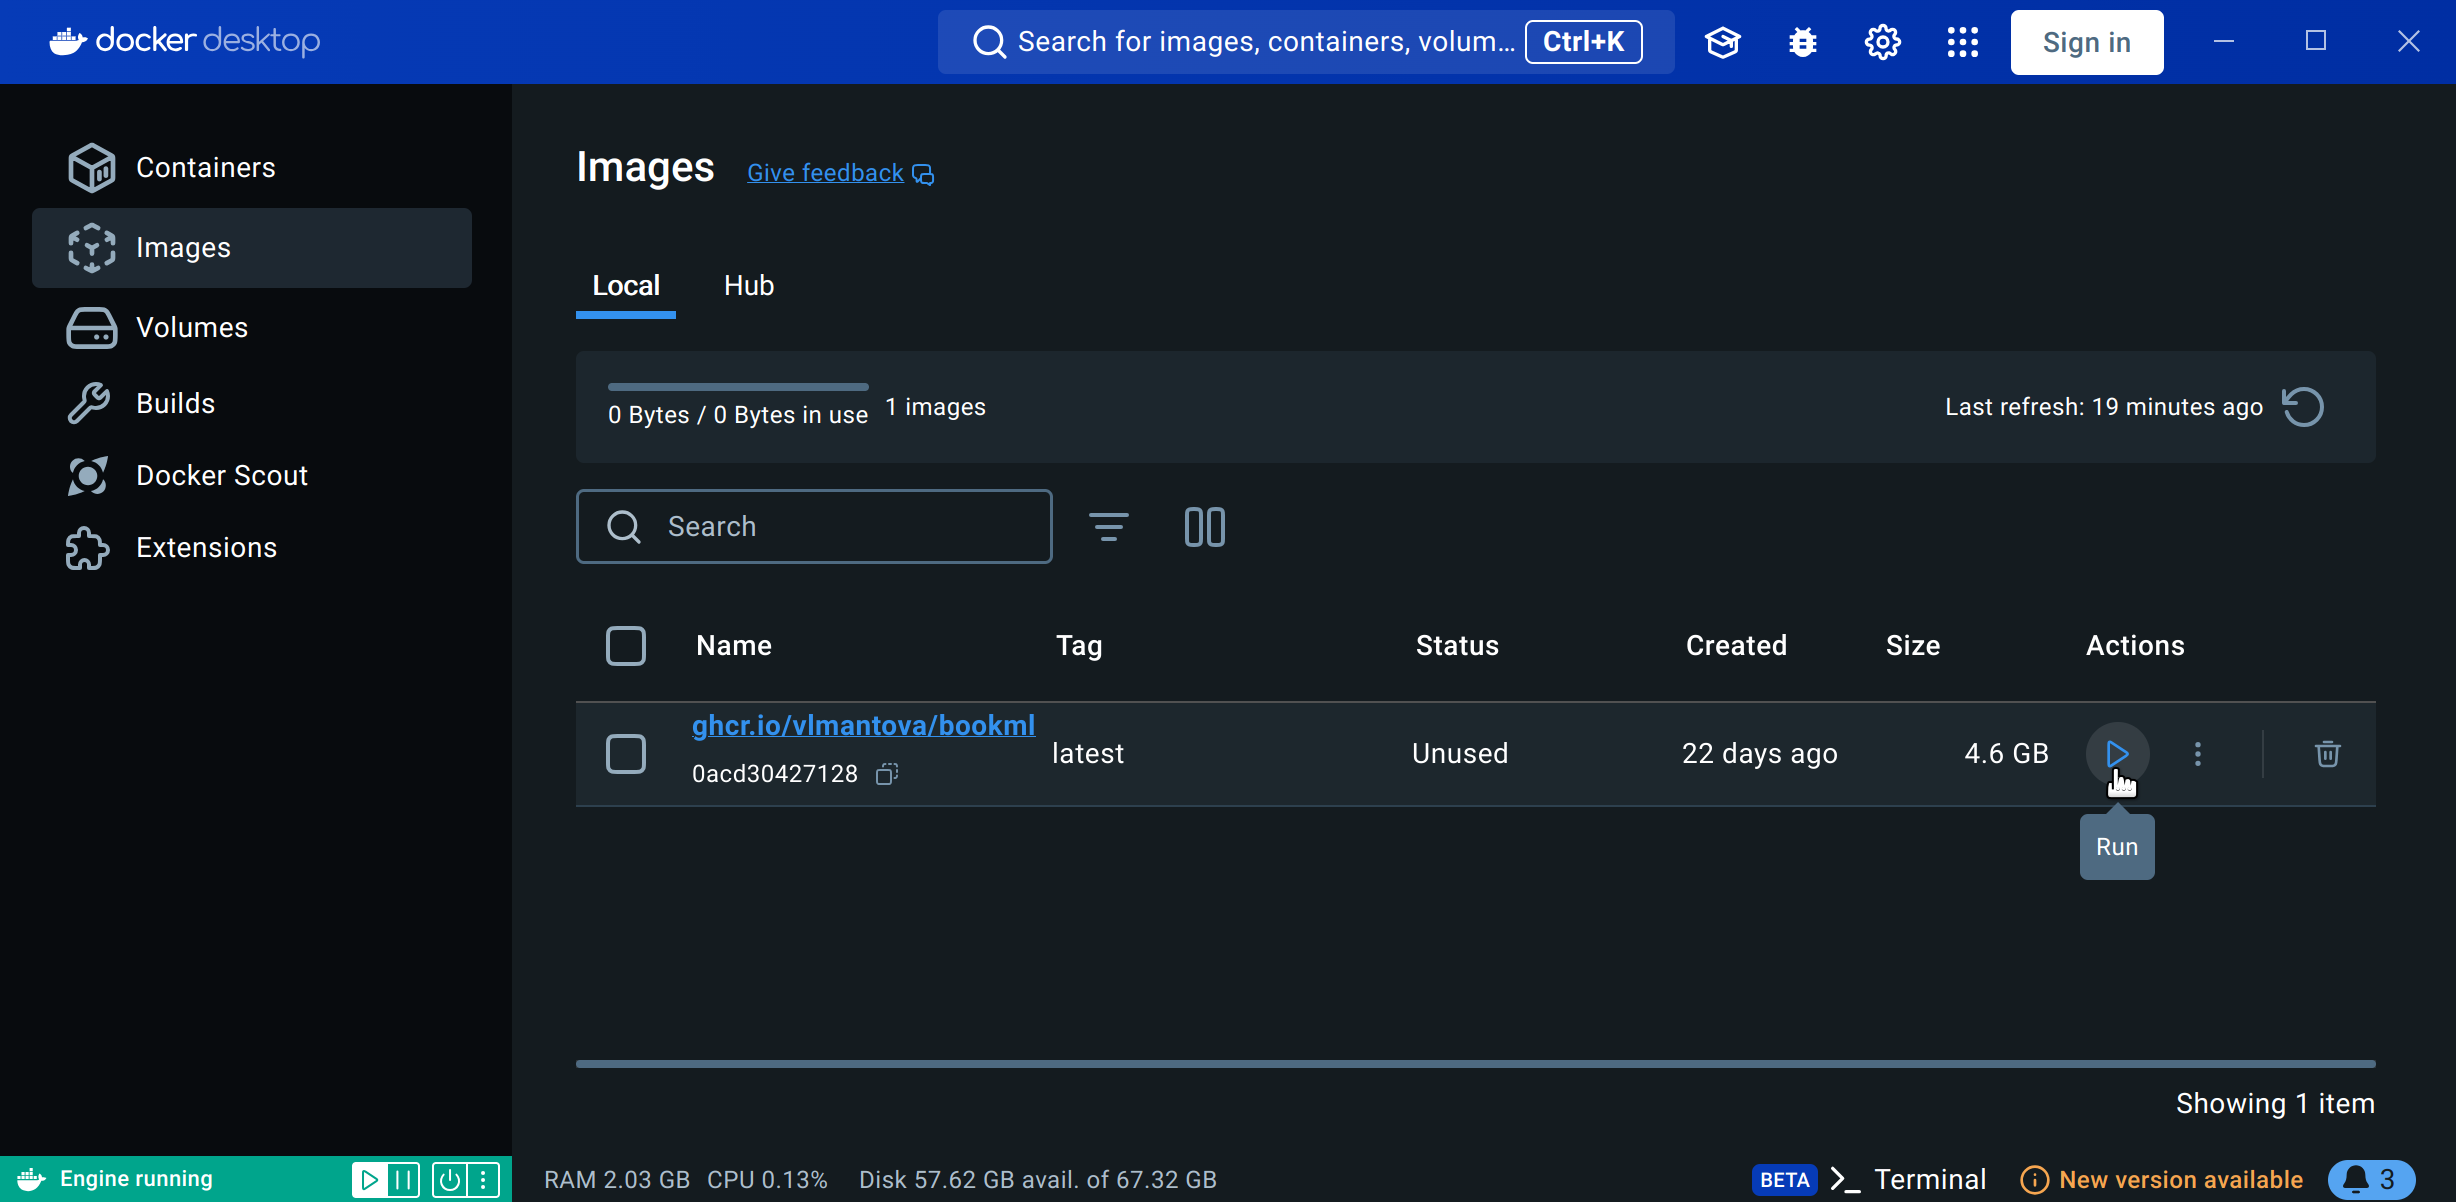
\includegraphics[width=\textwidth, alt={A screenshot of Docker Desktop, with the cursor placed on the ``Run'' button.}]{img/docker_desktop_run.png}
    \caption{Step 1: click the `play' button to run the command.}
    \label{fig:docker_desktop_run}
\end{figure}

\begin{figure}[h!]
    \centering
    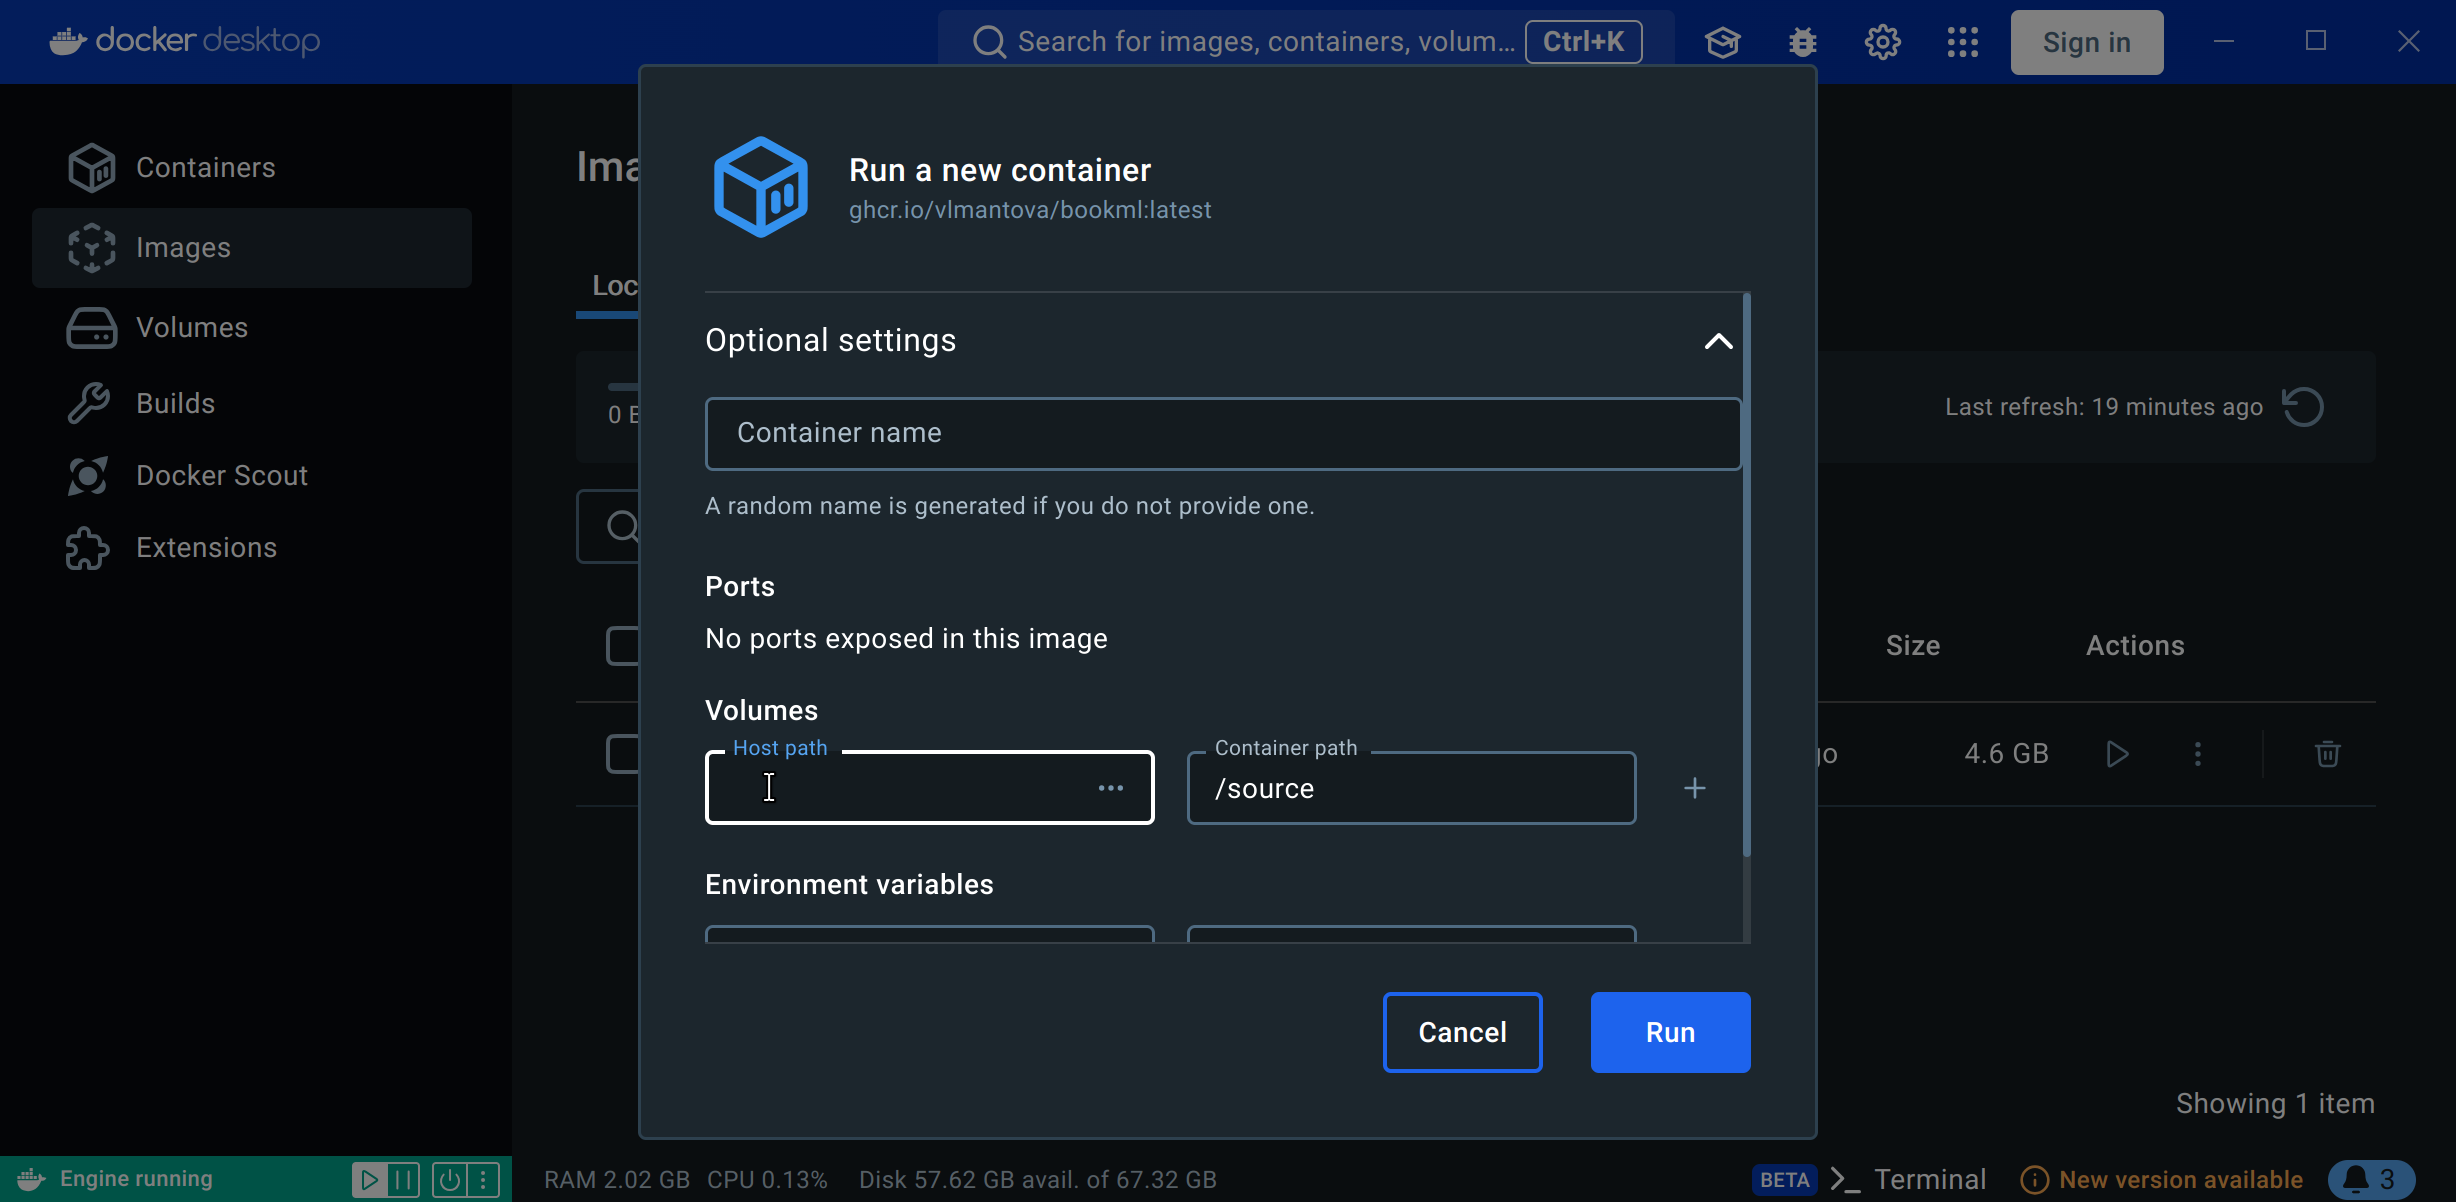
\includegraphics[width=\textwidth, alt={A screenshot of Docker Desktop, showing where to input the folder path.}]{img/docker_desktop_path.png}
    \caption{Step 2: give Docker the path to your folder.}
    \label{fig:docker_desktop_path}
\end{figure}

\subsection{Not using Docker}
\label{ssec:install}

If you prefer to install the necessary packages and dependencies to your machine, you can follow the instructions in the \href{https://vlmantova.github.io/bookmlleeds/#S1}{BookML documentation}.





Running BookML will produce PDF files (with \verb|pdflatex|), as well as \verb|.zip| files containing the HTML versions of your \verb|.tex| files, which can be uploaded directly to Learn. The output (both PDF and HTML) will be found in the same folder as your \verb|.tex| files.

To convert files locally (on your own machine), there are two options: installing the required packages and dependencies yourself, or using a Docker container. 
This image is 4.6GB so be prepared for a large download.
Whichever option you use, conversion is likely to take a few hours if you have large files (\(\approx\) 200 pages). 



\subsubsection{Upload SCORM}
\label{ssec:scorm}

The easiest way to upload the HTML materials to Learn is using the \verb|SCORM.myfolder.zip| which is created automatically.

\begin{itemize}
    \item On your Learn page, create a new content item.
    \item Choose the ``SCORM package'' option.
    \item Upload the file \verb|SCORM.myfolder.zip|.
    \item Once it's uploaded, untick the ``Mark SCORM'' checkbox, and click ``Save''.
\end{itemize}

\begin{figure}[h!]
    \centering
    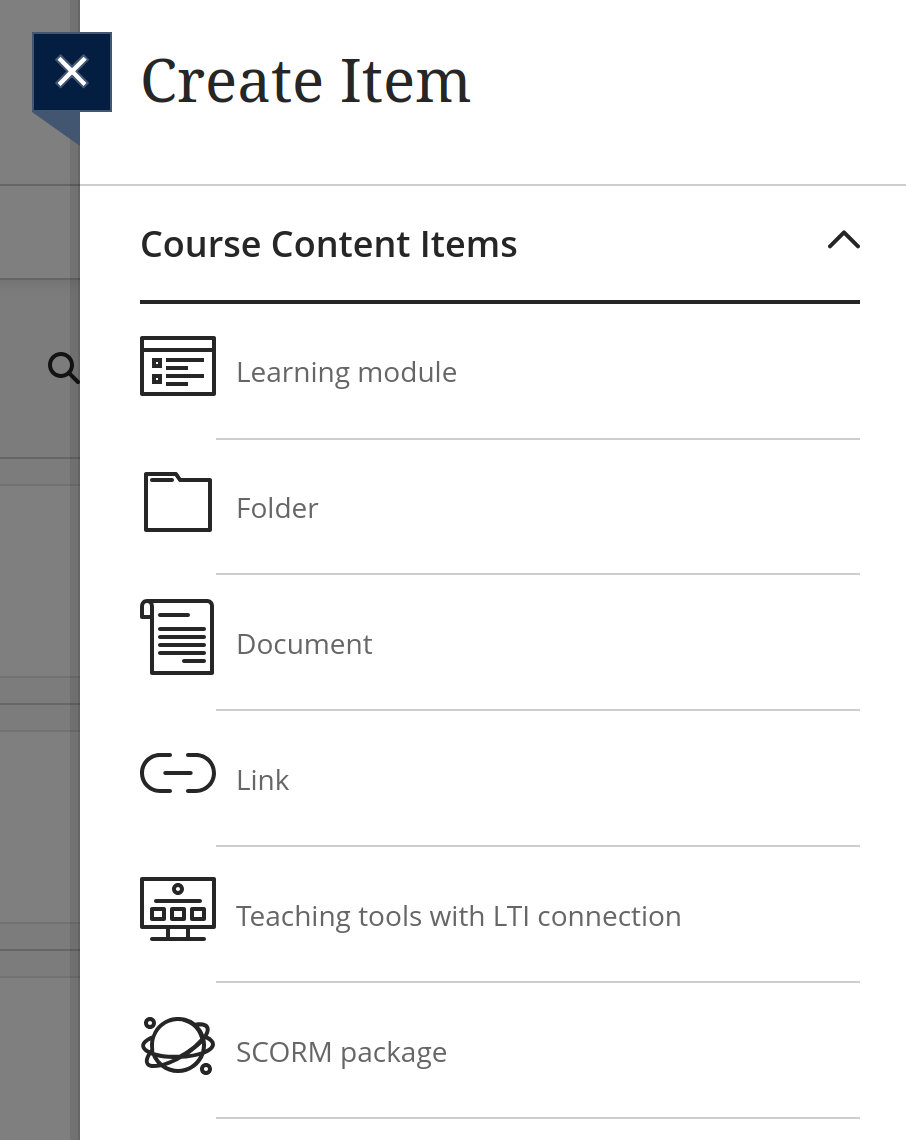
\includegraphics[width=0.5\textwidth, alt={A screenshot of the ``Create content'' menu on Learn Ultra showing different options. The last option is ``SCORM package''.}]{img/scorm.png}
    \caption{The ``SCORM package'' option on Learn Ultra.}
    \label{fig:scorm}
\end{figure}
 


\subsection{Learning Technology Mailbox}
\label{ssec:lt}

If you would rather, you can also email \verb|lt@maths.ed.ac.uk| with a .zip of the folder containing all your course materials (everything needed for your .tex files to compile normally). The Learning Technology team will perform the conversion, and email you back with a .zip file containing the HTML version of your course materials; optionally, they can also upload it to your Learn page. If they spot anything which didn't convert well, they will let you know.


\section{FAQs}
\label{sec:FAQ}


\begin{description}[style=nextline]
\item[Q: Error: \texttt{Warning: no .tex files with \textbackslash{}documentclass found in this directory}]

\textbf{A:} The software cannot reach your files, this may be due to running the software in the wrong place, permissions, or a remote directory. 
Double check your file path, and try moving the files to a local directory and try again.

\item[Q: The conversion process is taking a very long time.]

\textbf{A:} The conversion process can take a while, especially for larger documents --- but if it's 30 minutes or more, then please flag this. Note that, if you are using a local installation (not Docker), there are some known issues related to this:
    \begin{itemize}
        \item There is a \href{https://github.com/brucemiller/LaTeXML/issues/2268}{known issue} with the package \verb|expl3| when used with TeXlive 2022 and older which can cause the conversion to take longer.
        \item There is a known issue with the ``postprocessing XSLT'' stage taking several minutes (instead of seconds) on Ubuntu 22.04.
    \end{itemize}

\end{description}
 
\noindent\textbf{Q: Will my .tex files be converted if I comment out} \verb|\|\verb|documentclass|? 
\begin{ans}
    Yes, and it may cause errors. For files which you don't want to be converted standalone (e.g. files which are \verb|\input|ted into another file), delete the \verb|\|\verb|documentclass| command entirely or move them into a folder.
\end{ans}

\noindent\textbf{Q: Why aren't my files converting at all, there is not an error, BookML simply states there are no files to convert.} 
\begin{ans}
    This is likely due to the fact that the software cannot reach your files. This can be because your files are in a folder, or that your files have \href{https://stackoverflow.com/questions/1976007/what-characters-are-forbidden-in-windows-and-linux-directory-names}{forbidden file characters} or a space.
    
\end{ans}

\section{Other Accessibility Information}
\label{sec:otheraccessibility}

This is not the whole picture. There are other things to consider when creating accessible documents that is not handled by materials being in HTML. Additonally, there are other alternatives to a \LaTeX to HTML conversion. 

\subsection{Other Considerations}
\label{ssec:otheraccessibility}

\begin{itemize}
    \item \textbf{Images:} Ensure that all images have \textit{quality} alt text. This is not done automatically by BookML, so you will need to add this manually. Information on how to add alt text is in the demo portion of this document, with information about images.
    \item \textbf{Links:} Ensure that all link text is accessible.
    \item \textbf{Use of colour:} Colour should not be used to comunicate information. This is often missed in graphs and charts. For example, potions of a pie chart should be directly labeled or the legend should be texture based.
\end{itemize}

\subsection{Alternatives to BookML}
Instead of using BookML, you can create an accessible format such as HTML from the begining.
This can be done using software such as Rmarkdown or Quarto. With these formats you may wish to upload the produced HTML files to Learn. See instructions in \ref{appb:zip} for how to upload a zip file to Learn.

% \appendix
% \section{Docker from software centre}
% \label{app:a}
% This method is more complicated than the Docker Desktop download from the internet, but avoids need of admin privileges.
% \begin{enumerate}
    % \item Open the Software Centre and search for Docker Desktop.
    % \item Click on the Docker Desktop icon and click `Install'.
    % \item This download may give the message it has failed, click retry.
    % \item Repeat this a few times, between each download type `docker' into a terminal window and press enter.
     % If docker is installed, the terminal will return a long message about docker commands. If it is not, it will not recognise the command.
    % \item Eventually, the download will prompt a restart. Allow this.
    % \item At this point, leave the machine for an extended time, potentially overnight. 
    % \item After this time, open a terminal window and type `docker' and press enter. 
    % \item Install once again, and the download should be successful. Check using the terminal.
% \end{enumerate}
